\subsubsection{Page Object Model}

Page Object Model ist ein in Selenium verwendetes Entwurfsmuster,
bei dem ein Objektrepository zur Speicherung von WebElementen
erstellt wird. Es wird eine Java-Klasse erstellt, die jeder WebSeite
entspricht (siehe \Cref{fig:page-obj}). Diese Seiten bestehen aus WebElementen und den
entsprechenden Methoden, die auf diese Elemente einwirken (siehe \Cref{fig:page-exp}).
Alle Webseitenelemente befinden sich in einer Java-Klasse, indem sie durch
ihre Locators identifiziert werden.  Darüber hinaus werden für die
verschiedenen Seiten der Webseite mehrere Java-Klassen erstellt. Diese
Java-Klassen dienen als Repository, in dem die verschiedenen Elemente
gespeichert werden, mit denen Testfällen interagieren können. Die Verwendung
des Page Object Model hat viele Vorteile:

\begin{enumerate}
    \item \textbf{Erleichtert die Wartung des Codes} : Da die Testklassen von den
    Klassen getrennt sind, die die Webelemente und die Operationen auf
    ihnen enthalten, ist die Aktualisierung des Codes sehr einfach, wenn
    ein Webelement aktualisiert oder ein neues hinzugefügt wird.
    \item \textbf{Erleichtert die Lesbarkeit des Codes} : Der Benutzer kann das Projekt
    und die Testskripte aufgrund der feinen Trennung zwischen den Testklassen
    und den verschiedenen Webseiten leicht durchlesen.
    \item \textbf{Wiederverwendbarkeit des Codes} : Wenn mehrere Testskripte dieselben
    Webelemente verwenden, müssen wir nicht in jedem Testskript Code zur
    Behandlung des Webelements schreiben. Die Unterbringung in einer
    separaten Seitenklasse macht es wiederverwendbar, indem es von jedem
    Testskript aus zugänglich gemacht wird.
\end{enumerate}

\begin{figure}[H]
    \centering
    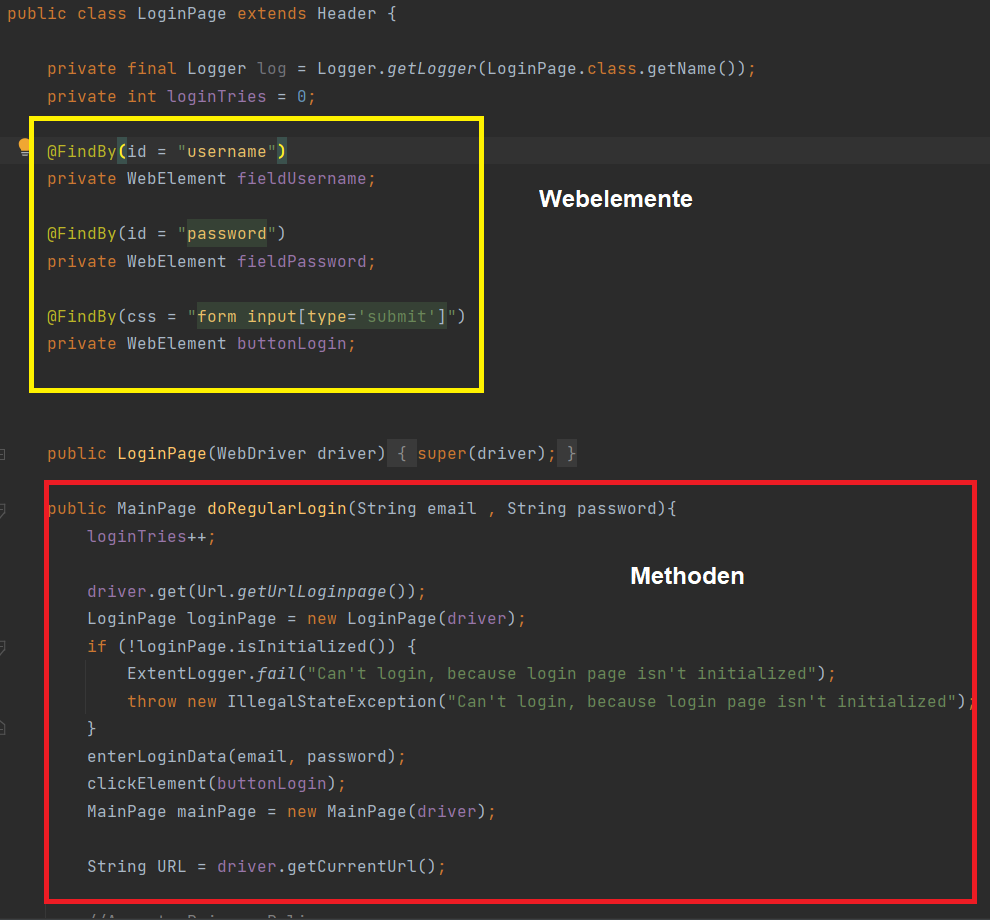
\includegraphics[scale=0.5]{images/page-example}
    \caption{Darstellung der JExam LoginPage mit dem Page Object Model} \label{fig:page-exp}
\end{figure}

\begin{figure}[H]
    \centering
    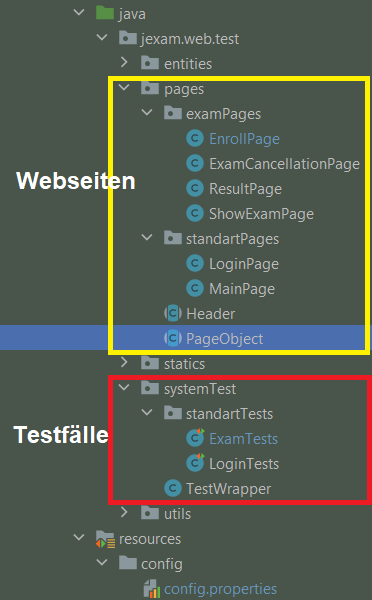
\includegraphics[scale=0.6]{images/page-object}
    \caption{Projektstruktur von jExam Page Object Model} \label{fig:page-obj}
\end{figure}
